\documentclass[12pt]{article}
\usepackage[english]{babel}
\usepackage[utf8x]{inputenc}
\usepackage{fullpage}
\usepackage{pythonhighlight}
\usepackage{graphicx}
\usepackage{geometry}
\usepackage{cite}
\usepackage{enumitem}
\usepackage{sectsty}
\usepackage[font=scriptsize,labelfont=bf]{caption}
\geometry{
	a4paper,
	top=0.89in,
	bottom=0.89in,
	left=0.9in,
	right=0.9in
}
% load package with some of the available options - you may not need this!
%\usepackage[framed,numbered,autolinebreaks,useliterate]{mcode}
\usepackage{titling}
\setlength{\droptitle}{-2cm}
\title{Project Report - Digit Classification}
\date{}
\author{\fontsize{12}{12}\selectfont Ce Zhang, Student No. 55542639\\
\fontsize{12}{12}\selectfont Yang Ji, Student No. 56064832}
\sectionfont{\fontsize{12}{12}\selectfont}

\begin{document}
\maketitle
\section{\fontsize{12}{12}\selectfont Introduction}
Modified National Institute of Standards and Technology (MNIST) is the standard dataset in the computation vision field. Since its release in 1999, this classical dataset, consisting of a collection of handwritten digit images, has been used extensively in machine learning and optical character recognition research. In real world, digit recognition system can significantly reduce the human effort and precisely recognize the digits from different resources like bank cheque, mails and drafts and in many demanding scenarios for numeric entries in tax forms, processing bank cheque amounts, recognizing number plates of vehicles and so on. 

In this project, we have a hands on experience of MNIST handwritten digital classification task,which is a branch of supervised learning. Given 4,000 images of handwriting digits, the task is to learn images' corresponding digits from 2,000 training images and evaluate machine learning methods with the left 2,000 test images. The number of training set is much smaller than the traditional MNIST benchmark's, where the training set contains 60,000 images. This makes our problem more challenging.

\section{\fontsize{12}{12}\selectfont Methodology}
Combining the learning algorithms studied in this course, we would like to pick suitable techniques in different parts of the entire machine learning task, ranging from feature selection to result evaluation.

\textbf{Step 1: Feature Selection} 
Since the raw data has been pre-processed to feature vectors, it removes the need of reading grey value of images, normalization and mean-subtraction by pixels and digits. Therefore, we take the first step to study Principal Component Analysis (PCA) and kernel Principal Component Analysis (kPCA) to speed up the following machine learning algorithms. PCA/kPCA is essentially a method that reduces the dimension of the feature space in such a way that new variables are orthogonal to each other. By generating these uncorrelated variables, we could make our trained classes more distinct when applying supervised classification methods. As for disadvantages, although PCA helps cover maximum variance among the features in a dataset, it might incur the loss of some information compared to the original features. In the implementation part, we leverage the PCA function in the Python library \textit{scikit-learn}.

\textbf{Step 2: Supervised Classification} 
In this part, we consider to evaluate: (1) logistic regression, (2) k-nearest-neighbor (kNN), (3) perceptron (4) SVM, (5) Simple Neural Network. Since some classifiers are binary classifiers, there are mainly two strategies that we can use: one versus all and one versus one. For one versus all method, the $i^{th}$ classifier is to separate the $i^{th}$ class with other $k-1$ classes, when we have $k$ classes. One versus one method is based on training $\frac{k(k-1)}{2}$ classifiers, where each classifier distinguishes two classes only. The class with more votes is selected as the output. We analyze the pros and cons of these four algorithms as follows.

\begin{enumerate}[label=(\roman*)]
	\item \textbf{Logistic Regression} 
	Logistic regression is a widely-used technique due to its efficiency and simplicity. It doesn't requires too many computing resources. It also removes the need of any tuning and scaling input data. What's more, it works better when removing unrelated or redundant attributes. However, it can't help solve non-linear problems due to its linear decision surface and can be easily outperformed by more complex ones.
	\item \textbf{kNN} 
	The main advantage of kNN is no training period when performing predictions. It means that new data can be added seamlessly which would not impact the final accuracy. But it doesn't work very well when dealing with large datasets or high-dimension datasets. What's more, kNN also requires to perform feature scaling (standardization and normalization) on the dataset. And kNN is also sensitive to noise in the dataset. The naive method to tackle this problem is to remove outliers manually.
    \item \textbf{Perceptron} 
	Like logistic regression, perceptron is also a widely-used technique due to its efficiency and simplicity. The difference between logistic regression and perception is the loss function. Perceptron just normally reflects the penalty is zero when correctly classified and would introduce large loss for large errors. Logistic Regression will introduce some small loss when correctly classified to push classification boundary away from points.
	\item \textbf{SVM} 
	SVM works relatively well when there is clear margin of separation between classes. It is more effective in the high dimensional spaces. However, iy might perform very well on large dataset or noisy dataset.
	\item \textbf{Neural Network} The simplest Neural Network is simply a multi-layer perceptron. It is good at modeling with non-linear data with large amount of training data. It is quite flexible that we can set any number of inputs and layers. However, its performance can be bad when we have limited training samples. Meanwhile, it often contains lots of hyperparameters, which brings the difficulty of tuning and explaining these parameters. 
\end{enumerate}

\section{\fontsize{12}{12}\selectfont Experimental Setup}
All of the experiments of the classical machine learning methods (kNN, SVM, Logistic Regression, Perceptron) are implemented using Python and the \emph{scikit learn} library. To make things easier, these methods are evaluated in a single file \emph{test.py}. Observing the datasets in \emph{digits4000\_txt} directory, there are total 4,000 images with corresponding labels. The training set and test set both include 2,000 images. All of the training tasks will be done with the 2,000 training images. For the accuracy computation, we leverage the \emph{score} method, provided by the \emph{scikit learn} library.

For each of the classical methods, we first evaluate the method using the raw training set. Then, different dimension reduction techniques like PCA, kPCA will be applied to the training set. Since the reduced dimension is a hyperparameter, we test different dimensions and try to find the optimal one. For SVM method, we also test the performance of different kernel functions since they can influence the classification performance.

For simple Neural Network, we leverage the widely used Keras library, which is based on the Tensorflow framework. We set three layers of the Neural Network: (1) First layer is the input layer and contains 500 neuron units with the ReLU activation function. (2) The second layer is the hidden layer, which also contains 500 neuron units and the activation function is also ReLU. (3) The last layer is the output layer, with 10 units and \emph{softmax} activation function. Since we have ten classes, we use the \emph{categorical\_crossentropy} and use one-hot encoding to transform the label to a 10 dimensional vector. To avoid the overfitting, we leverage the widely-used \emph{dropout} and each layers except for the output layer is added with a 0.5 \emph{dropout}.

%We use Python to check the class balance of the training images and finally find that each of the class contains 200 images. Therefore, our training set is very balanced in terms of all the classes.
\section{\fontsize{12}{12}\selectfont Experimental Results}
\subsection{kNN}
The accuracy of kNN algorithm with no data pre-processing is $\textbf{0.9135}$. To get better performance, we first apply PCA on the training set and we set the reduced dimension from 10 to 100. Fig.~\ref{fig:KNN-PCA} shows that $dim=40$ is the optimal reduced dimension. The best performance with PCA that we can get is $\textbf{0.931}$, which is better than the kNN without PCA. This means that by excluding the irrelevant features, we can get better performance for kNN algorithm. 
For kernel PCA (Fig.~\ref{fig:KNN-SIG-KPCA}, \ref{fig:KNN-RBF-KPCA}), sigmoid kernel PCA can slightly improve the accuracy, that is $\textbf{0.916}$ when dimension is 30. However, for rbf kernel, it makes the kNN performance even worse.
\begin{figure}[htpb]
	\centering
	\begin{minipage}{.3\textwidth}
		\centering
		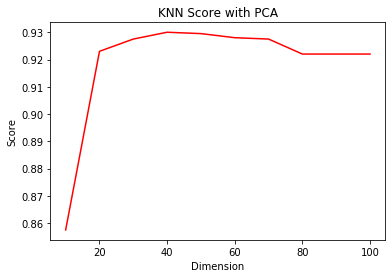
\includegraphics[width=\linewidth]{./exp-figs/KNN-PCA.png}
		\caption{KNN-PCA}
		\label{fig:KNN-PCA}
	\end{minipage}%
	\begin{minipage}{0.3\textwidth}
		\centering
		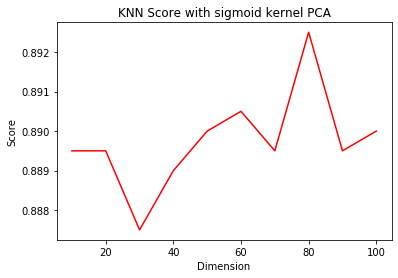
\includegraphics[width=\linewidth]{./exp-figs/KNN-SIG-KPCA.png}
		\caption{KNN-SIG-KPCA}
		\label{fig:KNN-SIG-KPCA}
	\end{minipage}
	\begin{minipage}{0.3\textwidth}
		\centering
		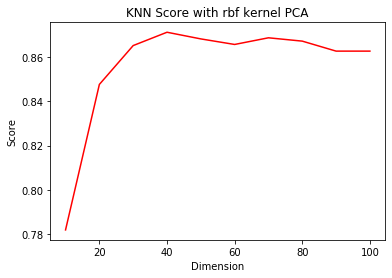
\includegraphics[width=\linewidth]{./exp-figs/KNN-RBF-KPCA.png}
		\caption{KNN-RBF-KPCA}
		\label{fig:KNN-RBF-KPCA}
	\end{minipage}
\end{figure}

\textbf{Performance Analysis} 

\begin{enumerate}[label=(\roman*)]
	\item By removing unrelated data, PCA can help evaluate kNN algorithm on the dataset with relatively low dimensions. 
	\item kPCA actually includes regular PCA as a special case. They're equivalent if the linear kernel is used. Despite capturing nonlinear structure in the dataset, kPCA which uses a nonlinear kernel might incur worse performance due to overfitting.
\end{enumerate}


\subsection{SVM}
In this section, we test the SVM performance. For SVM with polynomial kernel, the accuracy is $\textbf{0.9155}$, which is only slightly better than the kNN without PCA. However, if we change the kernel to RBF kernel, the accuracy is then $\textbf{0.941}$. This is even better than the kNN with PCA. This means that for SVM algorithm, the choice of kernel is quite important. We also test the SVM with \emph{decision\_function\_shape =ovo} and finally we get the same accuracy than the default \emph{ovr} setting.

To improve the performance of SVM, we apply the PCA to see whether it can help improve the accuracy. Observing Fig.~\ref{fig:SVM-PCA}, we can see that PCA can definitely improve the SVM's accuracy. When the dimension is 40, we get the optimum accuracy, that is $\textbf{0.9525}$. For kernel PCA, sigmoid PCA slightly improve the accuracy to $\textbf{0.942}$ when dimension is 30. However, for rbf kernel PCA, it hurts the performance for all tested dimensions.

\begin{figure}[htb]
	\centering
	\begin{minipage}{.3\textwidth}
		\centering
		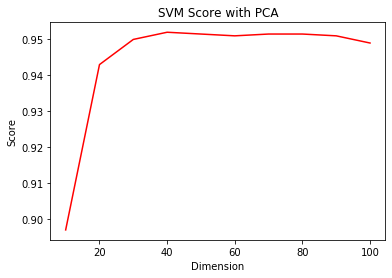
\includegraphics[width=\linewidth]{./exp-figs/SVM-PCA.png}
		\caption{SVM-PCA}
		\label{fig:SVM-PCA}
	\end{minipage}%
	\begin{minipage}{0.3\textwidth}
		\centering
		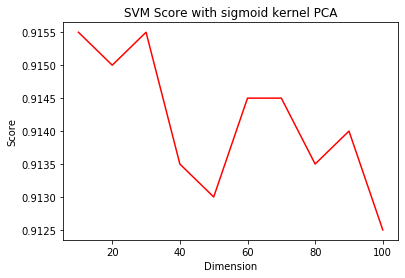
\includegraphics[width=\linewidth]{./exp-figs/SVM-SIG-KPCA.png}
		\caption{SVM-SIG-KPCA}
		\label{fig:SVM-SIG-KPCA}
	\end{minipage}
	\begin{minipage}{0.3\textwidth}
		\centering
		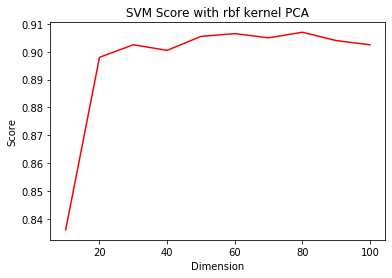
\includegraphics[width=\linewidth]{./exp-figs/SVM-RBF-KPCA.png}
		\caption{SVM-RBF-KPCA}
		\label{fig:SVM-RBF-KPCA}
	\end{minipage}
\end{figure}

\textbf{Performance Analysis} 

\begin{enumerate}[label=(\roman*)]
	\item Overall, SVM outperforms compared to the kNN since it tends to work well on a high-dimensional dataset.
	\item By removing unrelated data, PCA can help evaluate SVM algorithm on the dataset with relatively low dimensions. 
	\item Same as kNN-kPCA, the bad choice of kernel PCA might incur overfitting problems and decrease the generality of the trained model.
\end{enumerate}

\subsection{Logistic Regression}
In this section, we evaluate the performance of Logistic Regression. The accuracy of Logistic regression with raw data is $\textbf{0.8705}$, which is worse than both the kNN and also the SVM. Then, we use PCA to see whether we can improve the accuracy.

From Fig.~\ref{fig:LR-PCA}, we can see that the accuracy of Logistic Regression will first increase and then decrease with the increasing dimension. The highest accuracy of Logistic Regression with PCA is $\textbf{0.8785}$ when the dimension is 30. This accuracy is slightly higher than the one without PCA but is far more lower than both of the kNN and the SVM. However, both of the two kernel PCA methods decrease the accuracy.
\begin{figure}[htb]
	\centering
	\begin{minipage}{.3\textwidth}
		\centering
		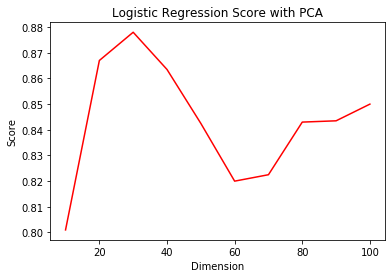
\includegraphics[width=\linewidth]{./exp-figs/LR-PCA.png}
		\caption{LR-PCA}
		\label{fig:LR-PCA}
	\end{minipage}%
	\begin{minipage}{0.3\textwidth}
		\centering
		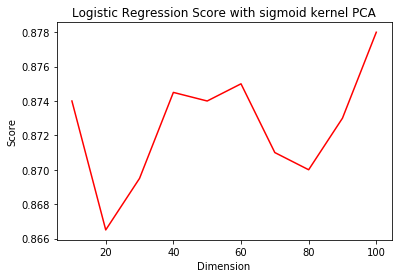
\includegraphics[width=\linewidth]{./exp-figs/LR-SIG-KPCA.png}
		\caption{LR-SIG-KPCA}
		\label{fig:LR-SIG-KPCA}
	\end{minipage}
	\begin{minipage}{0.3\textwidth}
		\centering
		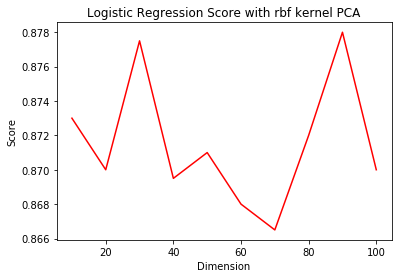
\includegraphics[width=\linewidth]{./exp-figs/LR-RBF-KPCA.png}
		\caption{LR-RBF-KPCA}
		\label{fig:LR-RBF-KPCA}
	\end{minipage}
\end{figure}

\textbf{Performance Analysis} 
\begin{enumerate}[label=(\roman*)]
	\item Overall, logistic regression under performs than kNN and SVM since it only works well on a linear dataset and can't tackle non-linear problems.
	\item The evaluation results also show that logistic regression can have a better performance when removing unrelated or redundant attributes. It is also why PCA/kPCA can help it improve the performance.
\end{enumerate}

\subsection{Perceptron}
For Perceptron method, the accuracy with raw data is $\textbf{0.8585}$, which is the lowest one among all of the above method. We also use PCA to see whether it can help improve the accuracy. However, according to Fig.~\ref{fig:P-PCA}, we can see that PCA hurts the accuracy of Perceptron. For sigmoid kernel PCA (Fig.~\ref{fig:P-SIG-KPCA}), we can see that when the dimension is 90, the accuracy is improved to $\textbf{0.867}$. But for rbf kernel PCA (Fig.~\ref{fig:P-RBF-KPCA}), it will not improve the accuracy of Perceptron in our experiment.

\begin{figure}[htb]
	\centering
	\begin{minipage}{.3\textwidth}
		\centering
		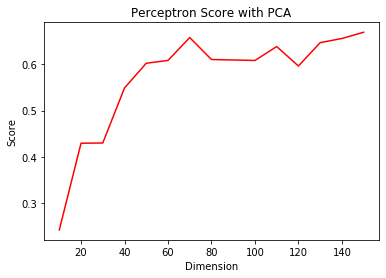
\includegraphics[width=\linewidth]{./exp-figs/P-PCA.png}
		\caption{Perceptron-PCA}
		\label{fig:P-PCA}
	\end{minipage}%
	\begin{minipage}{0.3\textwidth}
		\centering
		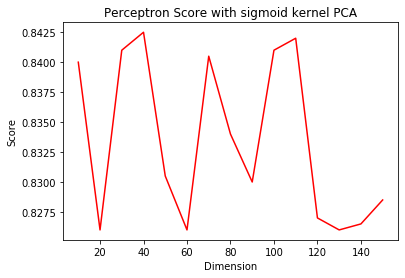
\includegraphics[width=\linewidth]{./exp-figs/P-SIG-KPCA.png}
		\caption{Perceptron-SIG-KPCA}
		\label{fig:P-SIG-KPCA}
	\end{minipage}
	\begin{minipage}{0.3\textwidth}
		\centering
		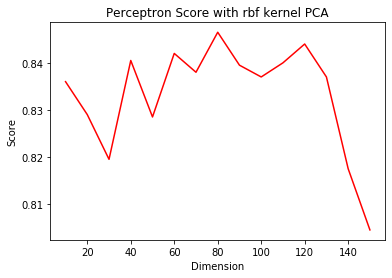
\includegraphics[width=\linewidth]{./exp-figs/P-RBF-KPCA.png}
		\caption{Perceptron-RBF-KPCA}
		\label{fig:P-RBF-KPCA}
	\end{minipage}
\end{figure}

\textbf{Performance Analysis} 
\begin{enumerate}[label=(\roman*)]
	\item Like logistic regression, perceptron has a relatively worse performance than SVM and kNN algorithm due to its linearity assumption.
	\item The choice of kernel may influence the test accuracy. Although the PCA/kPCA can help reduce the redundant information, they may also incur the loss of some information which leads to worse performance compared to perceptron without PCA/kPCA.
\end{enumerate}

\section{Simple Neural Network}
For three layer neural network, we train the network for 200 \emph{epochs}. The final test accuracy is $\textbf{0.846}$, which is worse than any of the classical algorithms without PCA. We find that the training accuracy reaches almost 1.0. Therefore, we know that the model is overfitting. This is because we have limited number of training data and Neural Network performs badly when the training data is not enough.

\begin{figure}[htb]
	\centering
	\begin{minipage}{.3\textwidth}
		\centering
		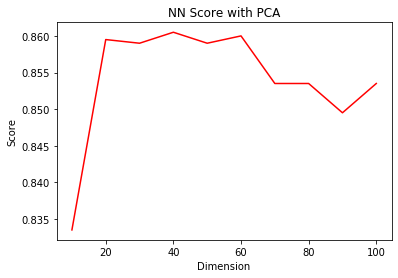
\includegraphics[width=\linewidth]{./exp-figs/NN-PCA.png}
		\caption{NN-PCA}
		\label{fig:NN-PCA}
	\end{minipage}%
	\begin{minipage}{0.3\textwidth}
		\centering
		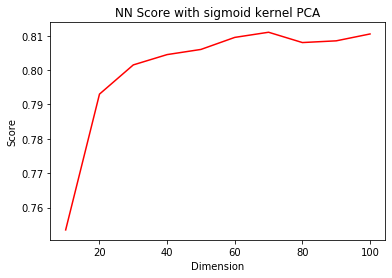
\includegraphics[width=\linewidth]{./exp-figs/NN-SIG-KPCA.png}
		\caption{NN-SIG-KPCA}
		\label{fig:NN-SIG-KPCA}
	\end{minipage}
	\begin{minipage}{0.3\textwidth}
		\centering
		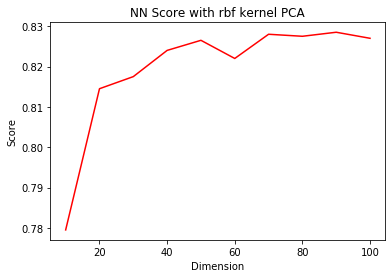
\includegraphics[width=\linewidth]{./exp-figs/NN-RBF-KPCA.png}
		\caption{NN-RBF-KPCA}
		\label{fig:NN-RBF-KPCA}
	\end{minipage}
\end{figure}

Then, we try to apply PCA and kernel PCA to see whether they can improve the accuracy. Observing Fig.~\ref{fig:NN-PCA}, we can see that when the dimension is 40, the accuracy is $\textbf{0.860}$, which is better than the Neural Network without PCA. But for both two cases of kernel PCA, none of them can improve the accuracy.

\textbf{Performance Analysis} 

\begin{enumerate}[label=(\roman*)]
	\item Simple three layer Neural Network's performance is worse than all of the classical machine learning algorithms. This is because the training set is too small and the test evaluation suffers from the great overfitting.
	\item PCA can help improve the accuracy since it can reduce the redundant information. However, the kernel PCA method hurts the accuracy since the bad choice of kernel might incur overfitting problems and decrease he generality of the model.
\end{enumerate}

\section{\fontsize{12}{12}\selectfont Appendix}
\begin{table}[htpb]
	\centering
	\caption*{\small{Summary of Used Algorithms}}
	\resizebox{.7\textwidth}{!}{% <------ Don't forget this %
		\begin{tabular}{|l|l|l|l|l|l|}
			\hline
			Method            & kNN    & SVM    & LR     & PCT       & NN    \\ \hline
			Acc               & 0.9135 & 0.941  & 0.8705 & 0.8585    & 0.846 \\ \hline
			Best PCA Acc      & 0.931   & 0.9525  & 0.8785  & 0.6765 & 0.8605 \\ \hline
			Best sig-kPCA Acc & 0.916 & 0.9435 & 0.8615  & 0.867     & 0.8110 \\ \hline
			Best rbf-kPCA Acc & 0.871  & 0.907  & 0.859 & 0.855      & 0.8285 \\ \hline
		\end{tabular}
	}
\end{table}
\bibliographystyle{IEEEtran}
%\bibliography{ref.bib}
\end{document}